%
% $XORP: xorp/docs/test_harness/test_harness.tex,v 1.36 2006/08/02 05:43:36 pavlin Exp $
%

\documentclass[11pt]{article}

%\usepackage[dvips]{changebar}

\usepackage{subfigure}
\usepackage{fullpage}
\usepackage{setspace}
\usepackage{times}
\usepackage{latexsym}
\usepackage{epsfig}
\usepackage{graphicx}
\usepackage{xspace}
\usepackage{color}
\usepackage{amsmath}
\usepackage{rotating}
\usepackage{moreverb}
\usepackage{listings}
\usepackage{alltt}
\usepackage{stmaryrd}
%\usepackage[dvipdf]{graphics}
%\usepackage[dvips]{graphicx}
%\usepackage{xorp}

\definecolor{gray}{rgb}{0.5,0.5,0.5}
\newcommand{\etc}{\emph{etc.}\xspace}
\newcommand{\ie}{\emph{i.e.,}\xspace}
\newcommand{\eg}{\emph{e.g.,}\xspace}
%\newcommand{\comment}[1]{{\color{gray}[\textsf{#1}]}}
%\newcommand{\comment}[1]{}

% Changebar stuff
% \newenvironment{colorcode}{\color{blue}}{}
% \renewcommand{\cbstart}{\begin{colorcode}}
% \renewcommand{\cbend}{\end{colorcode}}

% \pagestyle{empty}

\begin{document}

\title{XORP BGP Test Harness \\
\vspace{1ex}
Version 1.4}
\author{ XORP Project					\\
	 International Computer Science Institute	\\
	 Berkeley, CA 94704, USA			\\
         {\it http://www.xorp.org/}			\\
	 {\it feedback@xorp.org}
}
\date{March 20, 2007}

\maketitle


%%%%%%%%%%%%%%%%%%%%%%%%%%%%%%%%%%%%%%%%%%%%%%%%%%%%%%%%%%%%%%%%%%%%%%%
%
% Local definitions
%
\newcommand{\coordinator}{{\em coordinator}\xspace}
\newcommand{\testpeer}{{\em test peer}\xspace}
\newcommand{\testpeers}{{\em test peers}\xspace}

%%%%%%%%%%%%%%%%%%%%%%%%%%%%%%%%%%%%%%%%%%%%%%%%%%%%%%%%%%%%%%%%%%%%%%%
\section{Introduction}

This document describes a test harness that was built primarily to
test the XORP BGP implementation. It may be possible to augment the
harness to use it for testing other protocols.

A single BGP process is placed in the harness and tests
are performed on it. The tests can range from testing the decision
process to verifying that a session is dropped when the hold timer expires.

%%%%%%%%%%%%%%%%%%%%%%%%%%%%%%%%%%%%%%%%%%%%%%%%%%%%%%%%%%%%%%%%%%%%%%%
\section{Requirements}

A major requirement was to allow the testing of any BGP process, not
just our own. In the case of our own BGP process it was essential that
regression tests could be run and results verified totally from within
scripts, without the need for any manual configuration. The
XORP BGP regression tests can be run directly from the ``Makefiles''.
\newline

The test harness supports testing at various levels:

\begin{itemize}

  \item Decision process.

  The BGP decision process can be tested by sending update packets to
  BGP, then verifying that the correct update packets are sent by the
  BGP process to the other BGP peers. The actual packets sent by the
  BGP process can be compared to expected packets. 

  Another way that the BGP decision process can be tested is by
  testing the routing tables held at the peers.

  \item Low level testing.

  Testing responses to deliberately corrupted packets.

  \item Load testing. 

  Testing reaction to introducing a large number of routes back
  to back.

  \item Timer testing.

  Correct operation of timers such as the HOLD TIME timer.

\end{itemize}

%%%%%%%%%%%%%%%%%%%%%%%%%%%%%%%%%%%%%%%%%%%%%%%%%%%%%%%%%%%%%%%%%%%%%%%
\section{Usage}

\begin{figure}[htbp]
\centerline{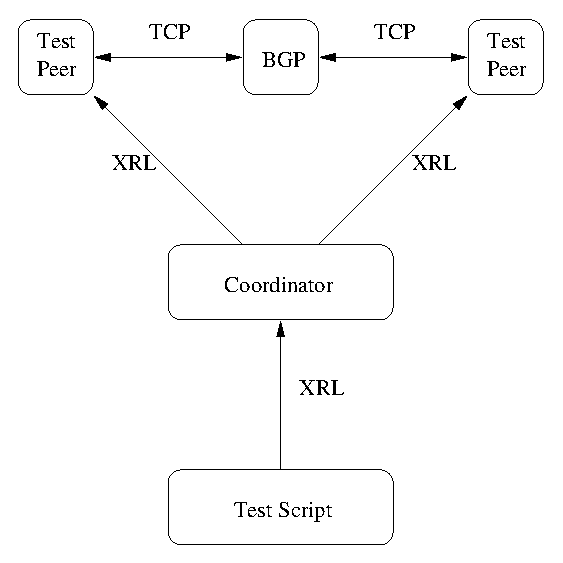
\includegraphics[width=0.70\textwidth]{figs/harness}}
\caption{\label{fig:harness}Test harness processes.}
\end{figure}

Figure \ref{fig:harness} shows a BGP process under test that is
connected to two test peers. The test harness has been split into a
number of separate processes. The main reason for using multiple
processes is that a third party BGP processes may not be able to
accept multiple connections from the same host (IP address). The
harness was also simpler to implement by splitting functionality into
separate processes.

The test harness consists of a \coordinator process through which
all interactions with the harness are mediated. There are also one or
more \testpeers . Each \testpeer is capable of forming one BGP
session with the BGP process under test. The \coordinator process
communicates with the \testpeers using XRLs \cite{xorp:xrl}. The
\coordinator process accepts commands via XRLs from test
scripts. Currently our test scripts are written in the shell
programming language, but they could be written in almost any
language. The full set of commands accepted by the \coordinator can be
found in \ref{coord:command}.

Figure \ref{prog:simple} shows an example of a simple program that
might be sent from a test script to a \coordinator. It is assumed that
before the script is sent that all the processes are already running.
One important point to note is that due to the asynchronous nature of
XRLs a command returning does not necessarily mean that it has
completed successfully. A {\em pending} method is available that can
be used to test if all outstanding commands have completed. This
example show the \coordinator being {\em reset}, then its given the
hostname and port number of the BGP process under test. Then the
\coordinator attaches to the two
\testpeers peer1 and peer2, these are the XRL target names by which the
\testpeers are known. The majority of the commands are sent to the
\testpeers themselves. In order to send a command to a \testpeer the
command is preceded by the \testpeer name. In our example each
\testpeer forms a session with the BGP process and then the
{\em assert} command is used to assert that a session is still
established. As noted above the {\em establish} command completing
does not mean that a session was established. Of course attempting to
send a {\em packet} on a session that has not yet been established
will generate an error.

\begin{figure}[htbp]
\small
\begin{verbatim}
reset
target xorp 179
initialise attach peer1
initialise attach peer2
peer1 establish active true AS 1 keepalive true holdtime 0 id 10.10.10.10
peer1 assert established
peer2 establish active true AS 2 keepalive true holdtime 0 id 20.20.20.20
peer2 assert established
\end{verbatim}
\caption{\label{prog:simple}Establish BGP Sessions}
\end{figure}

% An important and overloaded command is the {\em expect} command. Some
% of the commands that are performed by the {\em expect} command should
% really be performed by an {\em assert} command. Apart from the case of
% using {\em expect} to assert that a session has been established, all
% other cases of using {\em expect} are related to verifying that the
% BGP process under test has generated the correct sequence of
% packets.

The {\em expect packet \ldots} command is used to create a queue of
expected packets. Whenever a packet arrives on a peer it is checked
against the queue of expected packets. If there are no expected packets
on the queue then no action is taken. If there is a packet on the
expect queue it is compared against the incoming packet. If the
incoming packet matches,
all is fine and the packet is removed from the queue. If the incoming
packet does not match the packet at the head of the queue, then an
error is flagged and the non matching packet is saved. At the end of a
set of tests the {\em assert queue} command can be used to verify that
queue is at the expected length. If an error has occurred, this is the
point at which the non matching packet and the expected packet are
returned, along with an error status. Figure \ref{prog:assert} is a
example of a code fragment that is waiting for a notify packet on
peer1. A notify packet is added to the queue of expected
packets, then an update packet without an origin is sent to the BGP
process. An update packet without an origin is an error and should
generate the notify packet that is expected. Note that it is
the responsibility of test script to add a delay between sending the
{\em update packet} and the {\em assert}.

\begin{figure}[htbp]
\small
\begin{verbatim}
...
# Update error, missing well known attribute.
peer1 expect packet notify 3 3
# An update packet without an origin
peer1 send packet update aspath 1 nexthop 20.20.20.20 nlri 10.10.10.0/24
# Delay
peer1 assert queue 0
...
\end{verbatim}
\vspace{-0.1in}
\caption{\label{prog:assert}Wait for a notify packet}
\end{figure}

Each {\em peer} has two tries associated with it, a sent and a
received trie. Each update packet that is sent to, or received from,
the BGP process is passed to the appropriate trie. At this time two
types of {\em lookups} can be performed on a trie (Figure
\ref{prog:trie_lookup}). If a {\em lookup} fails then an error is
returned. A test might therefore involve sending many update packets
from different peers and then verifying that the routing tables at the
various peers are correct.  Saving the update packets in the tries
makes it possible to dump the routing tables for post processing.

\begin{figure}[htbp]
\small
\begin{verbatim}
...
peer1 trie recv lookup 212.174.196.0/24
peer1 trie recv lookup 212.174.196.0/24 aspath 1
...
\end{verbatim}
\vspace{-0.1in}
\caption{\label{prog:trie_lookup}Performing lookup in trie}
\end{figure}

%%%%%%%%%%%%%%%%%%%%%%%%%%%%%%%%%%%%%%%%%%%%%%%%%%%%%%%%%%%%%%%%%%%%%%%
\section{Commands}

%%%%%%%%%%%%%%%%%%%%%%%%%%%%%%%%%%%%%%%%%%%
\subsection{\label{coord:command}COORD XRLs}

\begin{itemize}

  \item Command("command string")

  Accept commands via XRLs.

  \item Status("peername")

  Returns the status of the named test peer. Can be used to detect if a
  peer is established or not. Plus the number of update messages sent
  or received by the peer. This XRL will not return an error if the
  requested peer does not exist. Can be used in test scripts to wait
  for established, not established transitions. As well as waiting for
  a peering to become quiet because all the state is
  synchronised.

  \item Pending()

  Returns true while there are any uncompleted commands. Can be used
  to poll the coordinator to verify that the previous command has
  completed.

\end{itemize}

%%%%%%%%%%%%%%%%%%%%%%
\subsubsection{Commands currently accepted by coord}

\begin{itemize}

  \item {\sf reset}

  Reset all the state in the coordinating process.

  \item {\sf target $<$hostname$>$ $<$port$>$}

  Specify the BGP process under test.

  \item {\sf initialise attach$/$create peername}

  Form an association with a test\_peer. If the second argument is attach then
  it is assumed that the test\_peer is already running. If the second
  argument is create then the test\_peer is started (not currently
  supported).

\end{itemize}

%%%%%%%%%%%%%%%%%%%%%%
\subsubsection{Peer specific commands}

\begin{itemize}

  \item connect

  Connect to the BGP target under test.

  \item disconnect

  Disconnect from the BGP target under test.

  \item listen 

  Listen for a connection from the BGP test target.

  \item {\sf establish
  active $<$true/false$>$
  AS $<$value$>$
  keepalive $<$true/false$>$
  holdtime $<$value$>$ 
  id $<$ipv4$>$}
  ipv6 $<$true/false$>$

  The active, AS, keepalive, holdtime, id and ipv6 arguments are
  optional. Active defaults to being true and actively makes a
  connection, setting active to false sets up a listener. The AS value
  is recommended if a connection is wanted. The ipv6 argument defaults
  to false.

  \item {\sf send packet update 
  origin $<$num$>$ 
  aspath $<$path$>$ 
  nexthop $<$ipv4$>$ 
  nexthop6 $<$ipv6$>$ 
  localpref $<$num$>$
  nlri $<$net4$>$
  nlri6 $<$net6$>$
  withdraw $<$net4$>$
  withdraw6 $<$net6$>$
  med $<$value$>$
  originatorid $<$ipv4$>$ 
  clusterlist $<$ipv4$>$ 
  community $<$community$>$
  pathattr $<$num,num,num,...$>$}

  Send a BGP update packet to the BGP test target with the specified
  withdrawn routes, NLRI, and path attributes. The ``pathattr''
  argument takes a list of commma separated byte values in decimal or
  hex. The ``patthattr'' exists to test optional path attributes. It
  should be noted that at this time it is not possible to create an
  illegal path attribute. The aspath can take the argument ``empty''
  denoting and empty aspath. The community can take either a number
  (in octal, decimal or hex)
  or the well known name ``NO\_EXPORT'', ``NO\_ADVERTISE'' or
  ``NO\_EXPORT\_SUBCONFED'', multiple communities can be added using
  multiple community statements. 

  \item {\sf send packet notify $<$error code$>$ $<$sub error code$>$}

  Send a notification packet. The $<$error code$>$ is mandatory. The
  $<$sub error code$>$ is optional.

  \item {\sf send packet keepalive}

  Send a keepalive packet.

  \item {\sf send packet open
                        asnum $<$value$>$ 
                        bgpid $<$ipv4$>$ 
                        holdtime $<$value$>$
			afi $<$value$>$
			safi $<$value$>$}

  Send an open packet.  All fields apart from afi and safi are mandatory.

  \item {\sf send packet corrupt $<$offset$>$ $<$value$>$ ... }

  Any of the packets listed above can be corrupted by preceeding with
  the corrupt keyword followed by an offset and value. The offset must
  fall within the packet, the offset starts from zero. Multiple offset
  value pairs may be used. An example of corrupting a keepalive can be
  seen in Figure \ref{prog:corrupt}.

\begin{figure}[htbp]
\small
\begin{verbatim}
...
peer1 send packet corrupt 0 0 keepalive
...
\end{verbatim}
\vspace{-0.1in}
\caption{\label{prog:corrupt}Corrupt a keepalive}
\end{figure}

  \item {\sf send dump mrtd update filename $<$packet count$>$}
  
  Given a file in mrtd dump format send the update packets in this
  file. Optionally supply a packet count for the number of update
  packets that should be sent.

  \item {\sf trie $<$recv/sent$>$ lookup $<$net$>$}

  Test to see if this net is in the test peer's send or receive trie.

  \item {\sf trie $<$recv/sent$>$ lookup $<$net$>$ not}

  Test to see if this net is not in the trie.

  \item {\sf trie $<$recv/sent$>$ lookup $<$net$>$ aspath $<$path$>$}

  Test to see if this net is in the trie and associated with the
  provided AS path. The AS path can be to the value ``empty'' if a
  check for an empty AS path is required.

  \item {\sf expect packet notify $<$error code$>$ $<$sub error code$>$}

  Place a notification packet on the expect queue. The $<$error code$>$ is
  mandatory. The $<$sub error code$>$ is optional.
  
  \item {\sf expect packet update 
                    origin $<$num$>$ 
                    aspath $<$path$>$ 
                    nexthop $<$ip$>$ 
                    localpref $<$num$>$
                    nlri $<$net$>$
                    withdraw $<$net$>$}

  Place an update packet on the expect queue. The aspath can take the
  argument ``empty'' denoting and empty aspath.

  \item {\sf expect packet open 
                        asnum $<$value$>$ 
                        bgpid $<$ipv4$>$ 
                        holdtime $<$value$>$}

  Place an open packet on the expect queue. All fields shown are mandatory.

  \item {\sf expect packet notify}

  Place a notify packet on the expect queue.

  \item {\sf assert queue $<$queue length$>$}

  Check the queue length of the expect queue. Every message that
  matches removes an entry from the queue. If an error has previously
  occurred then this call will return the error. The length of the
  queue check is optional.

  \item {\sf assert connected}

  Verify that a TCP session exists.

  \item {\sf assert established}

  Verify that a BGP session has actually been established. Some tests can pass
  without a BGP process being present. These tests require this interface.

  \item {\sf assert idle}

  Verify that no session is currently established. Useful for
  verifying that after an error the session has actually been torn down.

  \item {\sf dump $<$recv/sent$>$ $<$mtrd/text$>$ $<$ipv4/ipv6$>$ $<$traffic/routeview/replay/debug$>$ $<$filename$>$}

  A mechanism for saving conversations or dumping routing tables. The
  received and sent cases can be dealt with independently. Four types
  of dumps are supported:

  \begin{enumerate}

    \item Traffic.

    The is basically all the traffic which is sent and
    received. The dumping can be disabled by making a call with
    the $<$filename$>$ argument removed.

    \item Routeview.

    The current state of the routing table.

    \item Replay

    Trawls through the routing table and dumps all the update
    packets that have caused entries in the routing table. The
    packets are dumped in the order in which they arrived.

    \item Debug.

    Visit all nodes in the trie and dump the update packet that
    was responsible for this entry. Update packets can have
    multiple NLRI's associated with them so a packet can be in the
    dump many times.

  \end{enumerate}

  The save file can be either in mtrd dump format or in xorp text format.

\end{itemize}

%%%%%%%%%%%%%%%%%%%%%%%%%%%%%%%%%%%%%%%%%%%
\subsection{TEST PEER XRLs}

Commands that are accepted by the test peer. This interface is
used by the coordinating process to control the test peers. It should
never be used directly and is documented here for completeness.

\begin{itemize}
  \item Register("coord")
  
  This is an external registration to the test peer. All packets
  received by the test peer are sent to the "coord".

  \item Packetisation("bgp")
  
  Tell the test peer to treat incoming packets as BGP packets
  packetise them accordingly. Otherwise just packetise the the packets
  the way they appear from the connection.
        
  \item Connect("host", "port")

  Connect to the named host and port.

  \item Listen("address", "port")

  Listen for connections on this address and port.

  \item Bind("address", "port")

  Bind on this address and port. This command exists solely to test
  that the entity under test does not block in connect. It is not a
  requirement to make a call to ``bind'' before the ``connect'' or
  ``listen'' commands. 

  \item Send("Data")
  
  Send data on the TCP connection.        

  \item Disconnect()

  Drop the current TCP connection.

  \item Terminate()

  Terminate the process.

\end{itemize}

%%%%%%%%%%%%%%%%%%%%%%%%%%%%%%%%%%%%%%%%%%%
\subsection{TEST PEER CLIENT XRLs}

This interface is implemented by the coordinator which is a client of
the test peer.

\begin{itemize}
  \item Packet("peer", "status", "time", "data")

  \begin{itemize}
    \item "peer"
          
    The peer that the packet came from.

    \item "status" 

    If the remote peer had been asked to perform packetisation.
    Then if a bad message is received signify this. Also after a
    bad is received packetisation is disabled.

    \item "time"

    The time when the packet was received in micro seconds since
    \mbox{1970-1-1}.

    \item "data"
          
    The raw data that was read on the connection.

  \end{itemize}

\end{itemize}

%%%%%%%%%%%%%%%%%%%%%%%%%%%%%%%%%%%%%%%%%%%%%%%%%%%%%%%%%%%%%%%%%%%%%%%
\section{Outstanding Issues}

\begin{itemize}

  \item At the time of writing the harness has only been used against
  the XORP BGP process. There is no reason to believe that it could
  not be used against implementations.

\end{itemize}

%%%%%%%%%%%%%%%%%%%%%%%%%%%%%%%%%%%%%%%%%%%%%%%%%%%%%%%%%%%%%%%%%%%%%%%
%     APPENDIX
%%%%%%%%%%%%%%%%%%%%%%%%%%%%%%%%%%%%%%%%%%%%%%%%%%%%%%%%%%%%%%%%%%%%%%%
\appendix
\section{Modification History}

\begin{itemize}

  \item December 11, 2002: Initial version 0.1 completed.

  \item March 10, 2003: Updated to match XORP release 0.2: the ``med''
  argument is supported for building packets.

  \item June 9, 2003: Updated the version to 0.3, and the date.

  \item August 28, 2003: Updated to match XORP release 0.4.

  \item November 6, 2003: Updated to match XORP release 0.5.

  \item July 8, 2004: Updated to match XORP release 1.0.

  \item April 13, 2005: Updated to match XORP release 1.1: the ``afi'' and
  ``safi'' arguments are supported for building packets.

  \item March 8, 2006: Updated to match XORP release 1.2.

  \item August 2, 2006: Updated to match XORP release 1.3: added support for
  setting the community attribute in BGP update packets.

  \item March 20, 2007: Updated the version to 1.4, and the date.

\end{itemize}

%%%%%%%%%%%%%%%%%%%%%%%%%%%%%%%%%%%%%%%%%%%%%%%%%%%%%%%%%%%%%%%%%%%%%%%
%     BIBLIOGRAPHY
%%%%%%%%%%%%%%%%%%%%%%%%%%%%%%%%%%%%%%%%%%%%%%%%%%%%%%%%%%%%%%%%%%%%%%%
\bibliography{../tex/xorp}
\bibliographystyle{plain}

\end{document}
